% This is "aamas2014.tex", a revised version of aamas2013.tex
% This file should be compiled with "aamas2014.cls"
% This example file demonstrates the use of the 'aamas2014.cls'
% LaTeX2e document class file. It is for those submitting
% articles to AAMAS 2014  conference. This file is based on
% the sig-alternate.tex example file.
% The 'sig-alternate.cls' file of ACM will produce a similar-looking,
% albeit, 'tighter' paper resulting in, invariably, fewer pages.
% than the original style ACM style.
%
% ----------------------------------------------------------------------------------------------------------------
% This .tex file (and associated .cls ) produces:
%       1) The Permission Statement
%       2) The Conference (location) Info information
%       3) The Copyright Line with AAMAS data
%       4) NO page numbers
%
% as against the acm_proc_article-sp.cls file which
% DOES NOT produce 1) through 3) above.
%
% Using 'aamas2014.cls' you don't have control
% from within the source .tex file, over both the CopyrightYear
% (defaulted to 200X) and the IFAAMAS Copyright Data
% (defaulted to X-XXXXX-XX-X/XX/XX).
% These information will be overwritten by fixed AAMAS 2014  information
% in the style files - it is NOT as you are used with ACM style files.
%
% ---------------------------------------------------------------------------------------------------------------
% This .tex source is an example which *does* use
% the .bib file (from which the .bbl file % is produced).
% REMEMBER HOWEVER: After having produced the .bbl file,
% and prior to final submission, you *NEED* to 'insert'
% your .bbl file into your source .tex file so as to provide
% ONE 'self-contained' source file.
%

% This is the document class for full camera ready papers and extended abstracts repsectively

\documentclass{aamas2014}

% if you are using PDF LaTex and you cannot find a way for producing
% letter, the following explicit settings may help

\pdfpagewidth=8.5truein
\pdfpageheight=11truein

\usepackage[ruled, vlined]{algorithm2e}
\DontPrintSemicolon

\usepackage{graphicx}

\begin{document}

% In the original styles from ACM, you would have needed to
% add meta-info here. This is not necessary for AAMAS 2014  as
% the complete copyright information is generated by the cls-files.


\title{Mixed-Initiative Coordination for Disaster Response in the Real-World}

% AUTHORS


% For initial submission, do not give author names, but the
% tracking number, instead, as the review process is blind.

% You need the command \numberofauthors to handle the 'placement
% and alignment' of the authors beneath the title.
%
% For aesthetic reasons, we recommend 'three authors at a time'
% i.e. three 'name/affiliation blocks' be placed beneath the title.
%
% NOTE: You are NOT restricted in how many 'rows' of
% "name/affiliations" may appear. We just ask that you restrict
% the number of 'columns' to three.
%
% Because of the available 'opening page real-estate'
% we ask you to refrain from putting more than six authors
% (two rows with three columns) beneath the article title.
% More than six makes the first-page appear very cluttered indeed.
%
% Use the \alignauthor commands to handle the names
% and affiliations for an 'aesthetic maximum' of six authors.
% Add names, affiliations, addresses for
% the seventh etc. author(s) as the argument for the
% \additionalauthors command.
% These 'additional authors' will be output/set for you
% without further effort on your part as the last section in
% the body of your article BEFORE References or any Appendices.

%\numberofauthors{8} %  in this sample file, there are a *total*
% of EIGHT authors. SIX appear on the 'first-page' (for formatting
% reasons) and the remaining two appear in the \additionalauthors section.
%

\numberofauthors{1}

\author{
% You can go ahead and credit any number of authors here,
% e.g. one 'row of three' or two rows (consisting of one row of three
% and a second row of one, two or three).
%
% The command \alignauthor (no curly braces needed) should
% precede each author name, affiliation/snail-mail address and
% e-mail address. Additionally, tag each line of
% affiliation/address with \affaddr, and tag the
% e-mail address with \email.
% 1st. author
\alignauthor
Paper  XXX
%Ben Trovato\titlenote{Dr.~Trovato insisted his name be first.}\\
%       \affaddr{Institute for Clarity in Documentation}\\
%       \affaddr{1932 Wallamaloo Lane}\\
%       \affaddr{Wallamaloo, New Zealand}\\
%       \email{trovato@corporation.com}
% 2nd. author
%\alignauthor
%G.K.M. Tobin\titlenote{The secretary disavows any knowledge of this author's actions.}\\
%       \affaddr{Institute for Clarity in Documentation}\\
%       \affaddr{P.O. Box 1212}\\
%       \affaddr{Dublin, Ohio 43017-6221}\\
%       \email{webmaster@marysville-ohio.com}
% 3rd. author
%\alignauthor Lars Th{\o}rv{\"a}ld\titlenote{This author is the one who did all the really hard work.}\\
%       \affaddr{The Th{\o}rv{\"a}ld Group}\\
%       \affaddr{1 Th{\o}rv{\"a}ld Circle}\\
%       \affaddr{Hekla, Iceland}\\
%       \email{larst@affiliation.org}
}

%\and  % use '\and' if you need 'another row' of author names

% 4th. author
%\alignauthor Lawrence P. Leipuner\\
%       \affaddr{Brookhaven Laboratories}\\
%       \affaddr{Brookhaven National Lab}\\
%       \affaddr{P.O. Box 5000}\\
%       \email{lleipuner@researchlabs.org}

% 5th. author
%\alignauthor Sean Fogarty\\
%       \affaddr{NASA Ames Research Center}\\
%       \affaddr{Moffett Field}\\
%       \affaddr{California 94035}\\
%       \email{fogartys@amesres.org}

% 6th. author
%\alignauthor Charles Palmer\\
%       \affaddr{Palmer Research Laboratories}\\
%      \affaddr{8600 Datapoint Drive}\\
%       \affaddr{San Antonio, Texas 78229}\\
%       \email{cpalmer@prl.com}

%\and

%% 7th. author
%\alignauthor Lawrence P. Leipuner\\
%       \affaddr{Brookhaven Laboratories}\\
%       \affaddr{Brookhaven National Lab}\\
%       \affaddr{P.O. Box 5000}\\
%       \email{lleipuner@researchlabs.org}

%% 8th. author
%\alignauthor Sean Fogarty\\
%       \affaddr{NASA Ames Research Center}\\
%       \affaddr{Moffett Field}\\
%       \affaddr{California 94035}\\
%       \email{fogartys@amesres.org}

%% 9th. author
%\alignauthor Charles Palmer\\
%       \affaddr{Palmer Research Laboratories}\\
%       \affaddr{8600 Datapoint Drive}\\
%       \affaddr{San Antonio, Texas 78229}\\
%       \email{cpalmer@prl.com}

%}

%% There's nothing stopping you putting the seventh, eighth, etc.
%% author on the opening page (as the 'third row') but we ask,
%% for aesthetic reasons that you place these 'additional authors'
%% in the \additional authors block, viz.
%\additionalauthors{Additional authors: John Smith (The Th{\o}rv{\"a}ld Group,
%email: {\texttt{jsmith@affiliation.org}}) and Julius P.~Kumquat
%(The Kumquat Consortium, email: {\texttt{jpkumquat@consortium.net}}).}
%\date{30 July 1999}
%% Just remember to make sure that the TOTAL number of authors
%% is the number that will appear on the first page PLUS the
%% number that will appear in the \additionalauthors section.

\maketitle

\begin{abstract}
The problem of allocating emergency responders to rescue tasks is a key application area for agent-based coordination algorithms. However, to date, none of the proposed approaches take into account the uncertainty predominant in disaster scenarios and have been validated in a real-world deployment. Hence, in this paper, we propose a novel algorithm, using Multi-agent Markov Decision Processes to coordinate emergency responders and deploy this algorithm in a mixed-reality game to help an agent guide human players to complete rescue tasks. In our field trials, our algorithm is shown to improve human performance and our results allow us to elucidate some of the key challenges faced when  deploying of mixed-initiative team formation algorithms. \end{abstract}

% Note that the category section should be completed after reference to the ACM Computing Classification Scheme available at
% http://www.acm.org/about/class/1998/.

\category{H.4}{Information Systems Applications}{Multi-Agent Systems}

%A category including the fourth, optional field follows...
%\category{D.2.8}{Software Engineering}{Metrics}[complexity measures, performance measures]

%General terms should be selected from the following 16 terms: Algorithms, Management, Measurement, Documentation, Performance, Design, Economics, Reliability, Experimentation, Security, Human Factors, Standardization, Languages, Theory, Legal Aspects, Verification.

\terms{Design, Human Factors, Algorithms}

%Keywords are your own choice of terms you would like the paper to be indexed by.

\keywords{Human-Agent Interaction, Coordination, Decision under Uncertainty, Adjustable Autonomy}

\section{Introduction}
The coordination of teams of field responders in search and rescue missions is regarded as one  of the grand challenges for multi-agent systems research \cite{kitano}. In such settings, responders with different capabilities (e.g., fire extinguishing, digging, or life support) have to form teams in order to perform rescue tasks (e.g., extinguishing a fire or digging civilians out of rubble or both) to minimise  costs (e.g., time or money) and maximise the number of lives and buildings saved. Thus, responders have to plan their paths to the tasks (as these may be distributed in space) and form specific teams  to complete some tasks. These teams, in turn, may  need to disband and reform other teams to complete other tasks requiring different capabilities, taking into account the status (e.g., health or building fire) of the tasks and the environment (e.g., if a fire or radioactive cloud is spreading). Furthermore, uncertainty in the environment (e.g., wind direction or speed) or in the responders' abilities to complete tasks (e.g., some may be tired or get hurt) means that plans may need to change depending on the state of the players and the environment. 

To address these challenges, in recent years, a number of algorithms and mechanisms have been developed to create teams and allocate tasks. For example, \cite{ramchurn:teal:2010,koes:teal:2005,scerri:teal:200X} and \cite{ramchurn:robocup:2010,chapman:teal:2010}, developed centralised and decentralised optimisation algorithms respectively to allocate rescue tasks efficiently to teams of field responders with different capabilities. However, none of these approaches considered the uncertainty in the environment or in the field responders' abilities. Crucially, to date, while all of these algorithms have been shown to perform well in simulations (assuming agents as computational entities), none of them have been \emph{deployed} to guide \emph{real} human responders (amateur or expert) in real-time rescue missions. Thus, it is still unclear whether these algorithms will cope with real-world uncertainties (e.g., communication breakdowns or change in wind direction), be acceptable to humans (i.e., agent-computed plans are not confusing and take into account human capabilities), and do help humans perform better than on their own.

Against this background, in this paper we develop a novel algorithm for team coordination under uncertainty and evaluate it within a real-world mixed-reality game that embodies the simulation of team coordination in disaster response settings. In more detail, we consider scenario involving rescue tasks distributed in a disaster space over which a radioactive cloud is spreading. Tasks need to be completed by the responders before the area is completely covered by the cloud (as responders will die from radiation exposure) which is spreading according to varying wind speed and direction. Our algorithm captures the uncertainty in the scenario (i.e., in terms of environment and player states) and  is able to compute a policy to allocate responders to tasks to minimise the time to complete all tasks without them being exposed to significant radiation. The algorithm is then used by an agent to guide human responders based on their perceived states. This agent is then implemented in our deployed platform, AtomicOrchid, that structures the interaction between human responders, a human coordinator, and the agent in a mixed-reality location-based game. By so doing, we are able to study, both quantitatively and qualitatively, the performance of a mixed-initiative team (i.e., a human team under human and agent guidance)  and the interactions between the different actors in the system. Thus, this paper advances the state of the art in the following ways:
\begin{enumerate}
\item We develop a novel approximate algorithm for team formation under uncertainty using a Multi-agent Markov Decision Process (MMDP) paradigm, and show how it accounts for real-world uncertainties.
\item We present AtomicOrchid, a novel platform to evaluate team formation under uncertainty using the concept of mixed-reality games. AtomicOrchid allows an agent, using our team formation algorithm, to coordinate, in real-time, human players using mobile phone-based messaging, to complete rescue tasks efficiently.
\item We provide the first real-world evaluation of a team formation agent in a disaster response setting in field trials and present both quantitative and qualitative results. Our results allow us to elucidate some of the challenges for the formation of human-agent collectives, that is, mixed-initiative teams where control can be passed between agents and humans in flexible ways.
\end{enumerate}
When taken together, our results show, for the first time, how agent-based coordination algorithms for disaster response can be validated in the real-world. Moreover, these results allow us to derive a methodology and guidelines to evaluate human-agent interaction in real-world settings. 

The rest of this paper is structured as follows. Section \ref{sec:scenario} formalises the disaster response problem as an MMDP. Section \ref{sec:algorithm} then describes the algorithm to solve the path planning and task allocation problems presented by the MMDP while Section \ref{sec:atomic} describes the AtomicOrchid platform. Section \ref{sec:evaluation} presents our pilot study and the evaluation of the system in a number of field trials.  Finally, Section \ref{sec:conclusions} concludes.
\section{The Disaster Scenario}

\noindent We consider a disaster scenario involving a satellite, containing radioactive fuel, that has crashed in a sub-urban area (see Section \ref{atomic} to see how this helps implement a credible mixed-reality game). While debris is strewn around a large area, damaging buildings and causing accidents and injuring civilians, radioactive discharge from the debris is gradually spreading over the area, threatening to contaminate food reserves and people. Hence, emergency services, voluntary organisations, and the military are deployed to help evacuate the casualties and resources before these are engulfed by  radioactive cloud.  In what follows, we model this scenario formally and then describe the optimisation problem faced by the actors (i.e., including emergency services, volunteers, medics, and soldiers) in trying to save as many lives and resources as they can.

\subsection{Formal Model}
\noindent Let $G$ denote a grid overlaid on top of the disaster space, and the satellite and actors are located at various coordinates $(x,y) \in G$ in this grid. The set of field responders be denoted as $i_1, \cdots, i_n \in I$ and the set of rescue tasks as  $t_1,\cdots, t_m\in T$.  As responders enact tasks, they may become tired or get injured. Hence, we assign each responder  a health level $h_i\in [0,100]$. Moreover, each responder will have  a specific role  $r \in Roles$ (e.g., fire brigade, soldier, or medic) and this will determine the capabilities he or she has and therefore the tasks he or she can perform. We denote as $Roles(i)$ the role of responder $i$. In turn, to complete a given task $t$,  a set of responders $I' \subseteq I$ with specific roles $R_t \subseteq R$ is required. Thus, a task can only be completed by a team of responders $I'$ if $\{Roles(i) | i \in I'\} = R_t$. 

Given this model, we next formulate the optimisation problem faced by the responders (and later solved in Section \ref{sec:algo}). To this end, we propose a Multi-Agent Markov Decision Process (MMDP)~\cite{?} that captures the uncertainties of the radiative cloud and the responders' behaviours. Specifically, we model the spreading of the radiative cloud as a random process over the spatial space and allow the responders' actions to be failed or delayed during the rescue process. Other existing models for rescue tasks such as CFSTP~\cite{?} and HTSSC~\cite{?} cannot be applied to our problem as they usually require the process of task executions to be deterministic. They need to explicitly model the time limit of a task and the duration of completing a task by the responders as spatial and temporal constraints, which are stochastic in our domain. Instead, in the MMDP model, we represent the task executions as stochastic processes of state transitions. Thus, the uncertainties of the radiative cloud and the responders' behaviours can be straightforwardly captured with transition probabilities. Additionally, modeling the problem as a MMDP enables us to use many sophisticated algorithms that have already been developed in the literature.

\subsection{Radiation Cloud Modelling}\label{sec:radiation}
\noindent The radiation cloud is assumed to be monitored using a number of sensors on the ground (within the disaster space) that collect readings of the radiation cloud intensity and wind velocity every minute of the game. These sensors can be at fixed locations or held by mobile agents.  The radiation cloud diffusion process is modelled in a standard way by a nonlinear Markov field stochastic differential equation,  
\begin{eqnarray*}
\frac{D \text{Rad}({\bf z}, \tau)}{D \tau}=\kappa \triangledown^2 \text{Rad}({\bf z},\tau)-\text{Rad}({\bf z},\tau)\triangledown \cdot {\bf w}({\bf z},\tau)+\sigma({\bf z},\tau)
\end{eqnarray*}
where $D$ is the material derivative, $\text{Rad}({\bf z},\tau)$ is the radiation cloud intensity at location ${\bf z}$ at time $\tau$, $\kappa$ is a fixed diffusion coefficient and $\sigma$ is the radiation source(s) emission rate. The diffusion equation is solved on a regular grid defined across the environment with grid coordinates $G$ (as defined in Section \ref{sec:model}).  Furthermore, the grid is solved at discrete time instances $\tau$.  The cloud is driven by wind forces which vary both spatially and temporally.  These forces induce anisotropy into the cloud diffusion process which is proportional to the wind velocity, ${\bf w}({\bf z},\tau)$.  The wind velocity is drawn from two independent Gaussian processes (GP), one GP for each Cartesian coordinate axis, $w_i({\bf z},\tau)$, of ${\bf w}({\bf z},\tau)$.  The GP captures both the spatial distribution of the wind velocity and the dynamic process resulting from shifting wind patterns such as short term gusts and longer term variations. 

% In our simulation, each spatial wind velocity component is modelled by a squared-exponential GP covariance function, $K$, with fixed input and output scales (although any covariance function can be substituted). Furthermore, as wind conditions may change over time we introduce a temporal correlation coefficient, $\rho$, to the covariance function.  Thus, for a single component, $w_i$, of ${\bf w}$, defined over grid $G$ at times $\tau$ and $\tau^\prime$, the wind process covariance function is, $\text{Cov}(w_i(G,\tau),w_i(G,\tau^\prime))=\rho(\tau,\tau^\prime) K(G,G)$.  We note that, when $\rho=1$ the wind velocities are time invariant (although spatially variant).  Values of $\rho<1$ model wind conditions that change over time.

Using the above model, we are able to create a moving radiation cloud, thus posing a real challenge both for the HQ (agent and commander) and the responders on the ground, as predictions they can make of where the cloud will move to will be prone to uncertainty both to the simulated wind speed and direction. 


%(\textbf{Steve: in the platform we take the `real' values from the diffusion process i believe. Does the above capture this? We will say that we will add the features you mention below to a future version of the platform where we aim to do both situational awareness and rescue. Add a sentence above to conclude where we took the values from and the process takes into account the  location of radiation source. Also, your notation clashes with the notations in the scenario and Feng's algorithm - please try to align.}
%The cloud intensity and wind velocity are measured by {\it monitor agents} equipped with geiger-counters and anemometers.  These agents are directed to take measurements with greatest information gain in the radiation cloud intensity.  The measurements are folded into the EKF and this refines estimates of the radiation cloud across the grid.  Figure~\ref{radiation_screen_shots} shows example cloud simulations for slow varying (i.e. $\rho=0.99$) and gusty (i.e. $\rho=0.90$) wind conditions.  Figure~\ref{radiation_screen_shots}(a) shows slow varying wind conditions in which case the radiation cloud can be interpolated accurately using sparse sensor measurements and the LFM model.  Alternatively, during gusty conditions the radiation cloud model is more uncertain far from the locations where recent measurements have been taken, as shown in Figure~\ref{radiation_screen_shots}(b).
%
%\begin{figure}[ht] \begin{center}
%    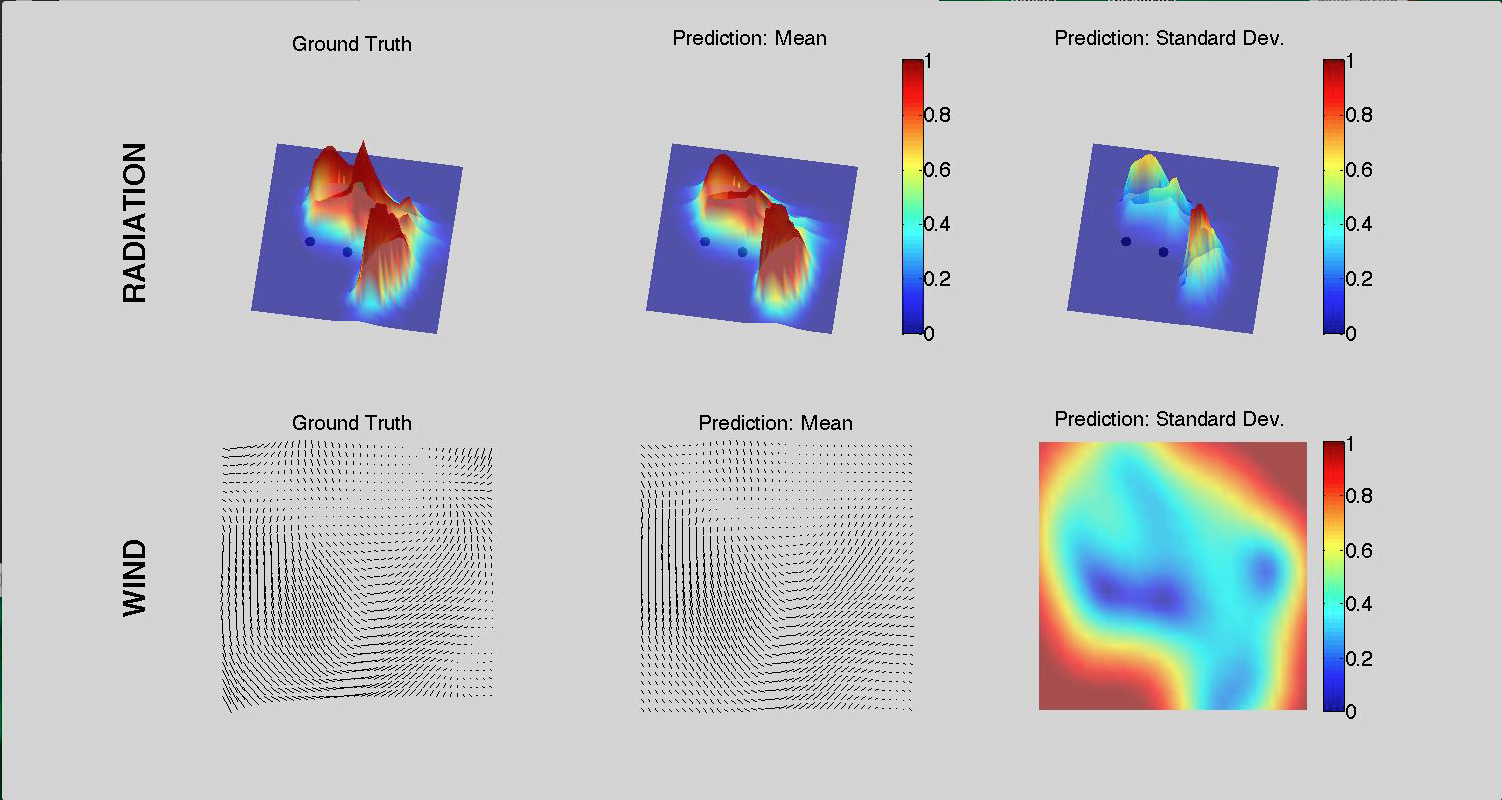
\includegraphics[width=0.45\textwidth]{figures/radiation_ss_calm.png}\\
%    (a) Slowly varying wind conditions\\ \ \\
%    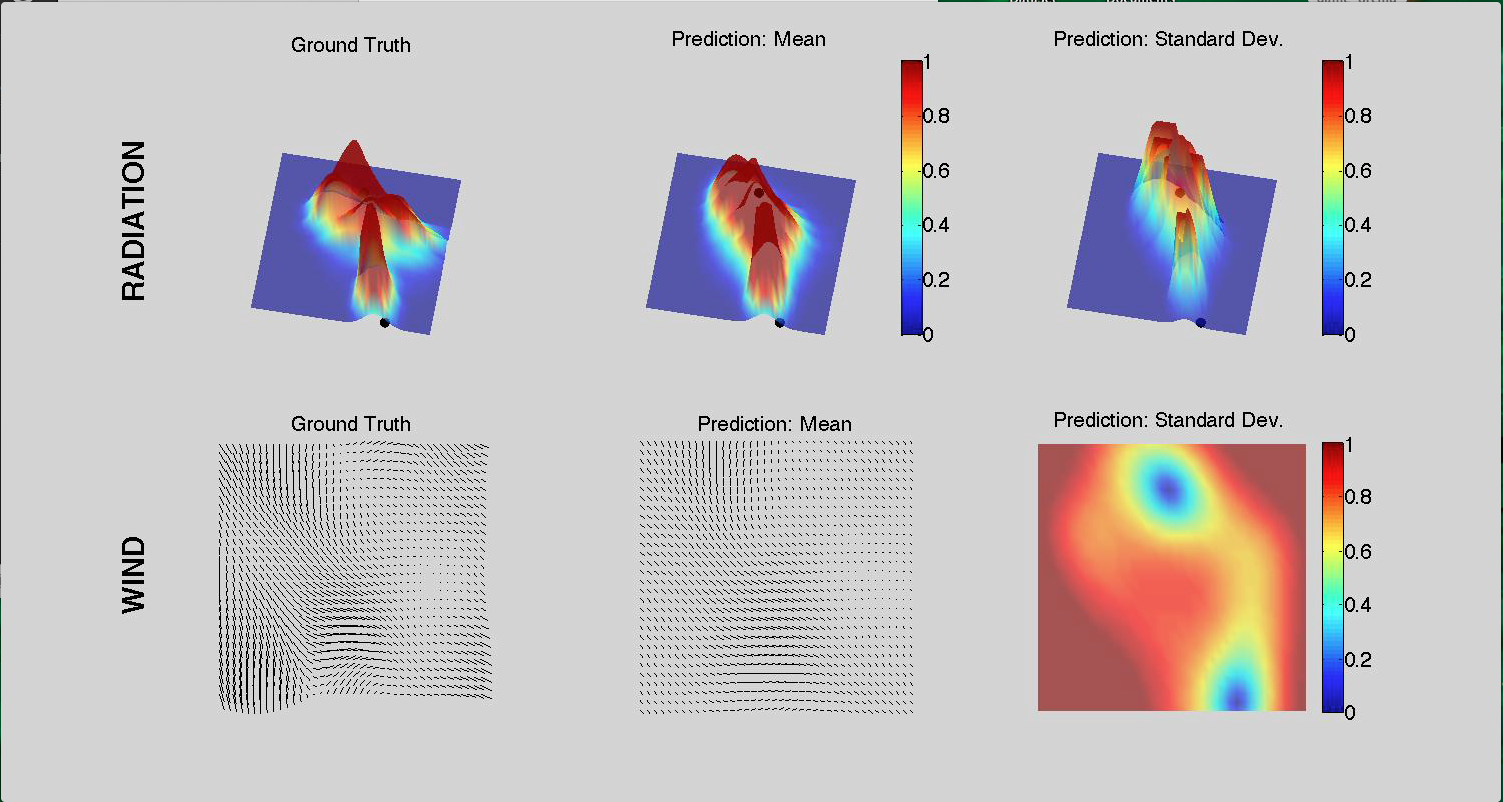
\includegraphics[width=0.45\textwidth]{figures/radiation_ss_gust.png}\\
%    (b) Gusty wind conditions 
%\caption{\label{radiation_screen_shots} Radiation and wind simulation ground truth and EKF estimates obtained using measurements from monitor agents (black dots).  Left most panes are ground truth radiation and wind conditions, the middle panes are corresponding estimates and right most panes are state uncertainties:  (a) Invariant and (b) gusty wind conditions.}
%\end{center}
%\end{figure}

\subsection{The Optimisation Problem}
\label{sec:model}
\noindent Previous agent-based models for team coordination in disaster response typically assume deterministic task executions and environments \cite{ramchurn:etal:2010,Scerri2005}. However, in order to evaluate agent-guided coordination in a real-world environment, it is important to consider uncertainties due to player behaviours and the environment (as discussed in the previous section). Given this, we propose a new representation for the task allocation problem in disaster response that does take into account such uncertainties. More specifically, we represent this problem using an MMDP that captures the uncertainties of the radioactive cloud and the responders' behaviours. We model the spreading of the radioactive cloud as a random process over the disaster space and allow the actions requested from the responders to  fail (because they decline to go to a  task) or incur delays (because they are too slow) during the rescue process. Thus in the MMDP model, we represent  task executions as stochastic processes of state transitions, while the uncertainties of the radioactive cloud and the responders' behaviours can be easily captured with transition probabilities.  More formally, the MMDP is
represented by tuple $\mathcal{M} = \langle I, S, \{A_i\}, P, R
\rangle$, where $I$ is the set of actors as defined in the previous
section,  $S$ is the state space, $A_i$ is a set of responder
$p_i$'s actions, $P$ is the transition function, and $R$ is the
reward function. We elaborate on each of these below.

In more detail, $S= S^G_r \times S_{p_1} \times \cdots \times
S_{p_n} \times S_{t_1} \times \cdots \times S_{t_m}$ where $S^G_r =
\{l_{(x,y)}| (x, y) \in G\}$ is the state variable of the
radioactive cloud that specifies the radioactive level
$l_{(x,y)}\in[0, 100]$ at every point $(x, y)\in G$. $S_{p_i} =
\langle h_i, (x_i, y_i), t_j \rangle$ is the state variable for
each responder $p_i$ that specifies her health level
$h_i\in[0, 100]$, her present position $(x_i, y_i)$, and the task
$t_j$ she is carrying out. $S_{t_j} = \langle {\tt st_j}, (x_j, y_j)
\rangle$ is then the state variable for task $t_j$ to specify its
status ${\tt st_j}$ (i.e., the target is picked up, dropped off, or idle) and position $(x_j, y_j)$. 

The three types of actions  (in set $A_i$) a responder can take
are: (i) {\em stay} in the current location $(x_i, y_i)$, (ii) {\em
move} to the 8 neighbouring locations, or (iii) {\em complete} a
task located at $(x_i, y_i)$. A joint action $\vec{a}=\langle a_1,
\cdots, a_n \rangle$ is a set of actions where $a_i\in A_i$, one
for each responder (a responder may just \emph{stay} at its current
position if it has no targets to rescue). The transition function
$P$ is defined in more detail as: $P= P_r \times P_{p_1} \times
\cdots \times P_{p_n} \times P_{t_1} \times \cdots \times P_{t_m}$
where:
\begin{itemize}
    \itemsep=-2pt
    \item $P_r(s'_r|s_r)$ is the probability the radioactive
        cloud spreads from state $s_r\in S^G_r$ to $s'_r\in
        S^G_r$. It captures the uncertainty of the  radiation
        levels in the environment due to  noisy sensor readings
        and the variations in wind speed and direction.
    \item $P_{p_i}(s'_{p_i}|s, a_i)$ is the probability
        responder $p_i$ transitions to a new state $s'_{p_i}\in
        S_{p_i}$ when executing action $a_i$. For example, when
        a responder is asked to go to a new location,  she
        may not end up there because  she is tired,
        gets injured, or receives radiation doses that are life
        threatening.
    \item $P_{t_j}(s'_{t_j}|s, \vec{a})$ is the probability
        of task $t_j$ being completed. A task $t_j$ can only be completed by a
        team of responders with the required types ($\Theta_{t_j}$) located at the
        same position as $t_j$.
\end{itemize}

Now,  if  $t_j$ is completed (i.e., in ${\tt st_j}\in S_{t_j}$, the
status ${\tt st_j}$ is marked as ``dropped off'' and its position $(x_j,
y_j)$ is within a safe zone), the team will be rewarded using
function $R$. The team is penalised if a responder $p_i$ gets
injured or receives a high dose of radiation (i.e., in $s_{p_i}$,
the health level $h_i$ is 0). Moreover, we attribute a cost to each
of the responders' actions since  each  action requires them to
exert some effort (e.g., running or carrying objects).


Give the above definitions, a policy for the MMDP is a mapping from
states to joint actions, $\pi: S \rightarrow \vec{A}$ so that the
responders know which actions to take given the current state of
the problem. The quality of a policy $\pi$ is  measured by
its expected value $V^\pi$, which can be computed recursively by
the Bellman equation:
\begin{equation}
  V^\pi(s^\tau) = R(s^\tau, \pi(s^\tau)) + \!\!\!\sum_{s^{\tau+1}\in S}\!\!\!
  P(s^{\tau+1}|s^\tau, \pi(s^t)) V^\pi(s^{\tau+1})
\end{equation}
where $\tau$ denotes the current time point and $\pi(s^\tau)$ is a joint action given $s^\tau$. The goal of solving
the MMDP is to find an optimal policy $\pi^*$ that maximises the
expected value with the initial state $s^0$, $\pi^* =
\arg\max_{\pi} V^\pi(s^0)$.

At each decision step, we assume the planning agent can fully
observe the state of the environment $s$ by collecting sensor
readings of the radioactive cloud and GPS locations of the
responders. Given a policy $\pi$ of the MMDP, a joint action
$\vec{a}=\pi(s)$ can be selected and broadcast to the responders
(as mentioned earlier).



\section{Team Coordination Algorithm}
Feng and Gopal
\begin{enumerate}
\item Feng's algorithm
\item experimental results in simulation - computational performance + no. of tasks completed in simulated settings. If possible, compare against something else.
\end{enumerate}

\section{Team Coordination Algorithm}
\label{sec:algo}
Although the MMDP model captures the uncertainties of our
problem, it results in a very large search space making it
practically impossible to compute the optimal solution. Hence, we consider approximate solutions that result in
high quality allocations. To this end, we decompose $PA$'s
decision-making process into a hierarchical planning process: at the top level, a {\em task planning} algorithm is run
for the whole team to assign the best task to each responder given
the current state of the world; at the lower level, given a task, a
{\em path planning} algorithm is run by each responder to find the
best path to the task from her current location. Furthermore,
since not all states of MMDPs are relevant to the problem, we
only need to consider the reachable states given the current state.
Hence, we compute the policy online, starting from the current state
of the problem. This reduces computation significantly
because the number of the reachable states is usually much smaller
than the overall state space. In what follows, we describe each
level of our {\em online hierarchical planning} algorithm.

\subsection{Task Planning} \label{sec:taskplanning} As described earlier, each responder $p_i$ is of a specific type
$\theta_i \in \Theta$ that determines which task she can perform
and  a task $t$ can only be completed by a team of responders with
the required types $\Theta_t$. If, during the execution
of a plan, a responder $p_i$ is incapable of performing a task
(e.g., because she is tired or unclear where the task is), she
is removed from the set of responders under consideration
(that is $I \to I \setminus p_i$). This information can be obtained
from the state $s \in S$. When a task is completed by a chosen
team, the task is simply removed from the set (that is $T \to
T\setminus t_k$ if $t_k$ has been completed).

Now, to capture the efficiency of groupings of responders at
performing tasks, we define the value of a team $v(C_{jk})$ that
reflects the level of performance of team $C_k$ in performing task
$t_j$. This is computed from the estimated rewards that the team
obtains for performing $t_j$.  Then, the goal of the task planning
algorithm is to assign a task to each team that maximises the
overall team performance given the current state $s$, i.e.,
$\sum_{j=1}^m v(C_{j})$ where $C_j$ is a team for task $t_j$ and
$\{ C_1, \cdots, C_m \}$ is a {\em partition} of $I$ ($\forall
j\neq j', C_j \bigcap C_{j'} = \emptyset$ and $\bigcup_{j=1}^m
C_j=I$). In what follows, we first detail the procedure to compute
the value of all teams that are valid in a given state and then
detail the task allocation algorithm.


\subsubsection{Team Value Calculation}
The computation of  $v(C_{jk})$ for each team $C_{jk}$ is
challenging since there are many ways to configure teams and this needs to be done repeatedly (since there are more tasks than responders).
Moreover, a new policy must be computed after a given task $t_j$ is completed. This is time-consuming given the number of
states and joint actions. Hence, we propose to estimate
$v(C_{jk})$ through several simulations. This saves
computation as it avoids computing the complete policy to come
up with a good estimate of the team value, though we may not be
able to evaluate all possible future outcomes. According to the
central limit theorem, if the number of simulations is sufficiently
large, the estimated value will converge to the true $v(C_{jk})$.

Specifically, in each simulation, we first assign the responders in
$C_{jk}$ to task $t_j$ and run the simulator starting from the
current state $s$. After task $t_j$ is completed, the simulator
returns the sum of the rewards $r$ and the new state $s'$. If all
the responders in $C_{jk}$ are incapable of doing other tasks
(e.g., suffered radiation burns), the simulation is terminated.
Otherwise, we estimate the expected value of $s'$ using Monte-Carlo
Tree Search (MCTS)~\cite{kocsis2006bandit}, which provides a good
trade-off between exploitation and exploration of the policy space
and has been shown to be efficient for large MDPs.\footnote{Other
methods such as sequential greedy assignment or swap-based hill
climbing~\cite{proper2009solving} may also be useful. However, they
do not explore the policy space as well as MCTS.} After $N$
simulations, the average value is returned as an approximation of
the team value.

\subsubsection{Coordinated Task Allocation}
Given the team values computed above, we then solve the following
optimisation problem to find the best solution:
\begin{equation}
  \begin{array}{lll}
    \max\limits_{x_{jk}} & \sum_{j, k} x_{jk} \cdot v(C_{jk}) & \\[2pt]
    \mbox{s.t.} & x_{jk} \in \{0, 1\} & \\[2pt]
    & \forall j, \sum_{k} x_{jk} \leq 1 & \mbox{(i)} \\[2pt]
    & \forall i, \sum_{j, k} \delta_i(C_{jk}) \leq 1 & \mbox{(ii)}
  \end{array}
  \label{eq:cf}
\end{equation}
where $x_{jk}$ is the boolean variable to indicate whether team
$C_{jk}$ is selected for task $t_j$ or not, $v(C_{jk})$ is the
value of team $C_{jk}$, and $\delta_i(C_{jk}) = 1$ if responder
$p_i\in C_{jk}$ and 0 otherwise. In the optimisation, constraint
(i) ensures that a task $t_j$ is allocated to at most one team (a
task does not need more than one group of responders) and
constraint (ii) ensures that a responder $p_i$ is assigned to only
one task (a responder cannot do more than one task at the same
time). This is a standard {\em mixed integer linear program} that
can be efficiently solved using solvers (e.g., CPLEX).

\subsubsection{Adapting to Responder Requests}\label{sec:adaptive}
An important characteristic of our approach is that it can easily
incorporate the preferences of the responders. For example, if a
responder declines a task allocated to it by the planning agent, we
simply filter out the teams for the task that contain this
responder. By so doing, the responder will not be assigned to the
task. Moreover, if a responder prefers to do the tasks with another
responder, we can increase the weights of the teams that contain
them in Equation~\ref{eq:cf} (by default, all teams have identical
weights of 1.0). Thus, our approach is adaptive to the
 preferences of human responders.\vspace{-2mm}

\subsection{Path Planning}
\label{sec:pathplanning}
In the path planning phase, we compute the best path for a
responder to her assigned task. This phase is stochastic due to uncertainties in the radioactive cloud and the responders'
actions. We model this problem as a single-agent MDP that can be
solved by many existing solvers. Among them, we choose {\em
real-time dynamic programming} (RTDP)~\cite{barto1995learning}
because it is simple and particularly fits our problem, that is, a
goal-directed MDP with large number of states. However, other
approaches for solving large MDPs  could equally be used here.

\subsection{Simulation Results}
While our main focus in this paper is the evaluation of our planning agent in the real-world, it is important  to ensure it
performs better than  greedy or myopic methods (particularly, given there is no extant solution that takes into account
uncertainty in team coordination for emergency response in the way we do).  In
the greedy method, the responders are uncoordinated and select the
closest tasks they can do. In the myopic method, the responders are
coordinated to select the tasks but have no lookahead for the
future tasks. For each method, we use our
path planning algorithm to compute the path for each responder.

Table~\ref{tab:simulation} shows the results for a problem with 17
tasks and 8 responders on a 50$\times$55 grid. As can be seen, our
MMDP algorithm completes more tasks than the myopic and greedy
methods (see Table \ref{tab:simulation}). More importantly, our
algorithm guarantees the safety of the responders (i.e., by avoiding the radioactive cloud), while in the
myopic method  only 25\% of the responders survive and in the
greedy method none survived.
More extensive evaluations are beyond the scope of this paper as
our focus here is on the use of the algorithm in a field deployment
to test how humans take up advice computed by the planning agent
$PA$.\vspace{-2mm}
\begin{table}[htbp]
\begin{center}\small
  
  \begin{tabular}{l|c|c|c}
   & MMDP & myopic & greedy \\
  \hline
  \#completed tasks & 71\% & 65\% & 41\% \\
  \hline
  \#responders alive at the end & 100\% & 25\% & 0\% \\
  \end{tabular}
  \end{center}\caption{Simulation results for MMDP, myopic, and greedy.}
  \label{tab:simulation}\vspace{-4mm}
\end{table}


\section{The Atomic Orchid Platform}
Joel and Wenchao
\begin{enumerate}
\item explain the main components  and how agent is integrated
\item explain the instructions given to participants and how it mimics the disaster response problem detailed above.
\end{enumerate}
\subsection{Game scenario}
AtomicOrchid is a location-based mobile game based on the fictitious scenario of radioactive explosions creating expanding and moving radioactive clouds that pose a threat to responders on the ground (the field players), and the targets to be rescued around the game area. Field responders are assigned a specific role (e.g. `medic', `transporter', `soldier', `ambulance') and targets have specific role requirements, so that only certain teams of responders can pick up certain targets. For example, an `injured person' can only be picked up by an `ambulance' and a `medic' together. To pick up targets, the team must be collocated in the immediate proximity of the geofenced target. Furthermore, field responders must not expose themselves to radioactivity from the cloud for too long, else they risk becoming `incapacitated'.

In their mission to rescue all the targets from the radioactive zone, the field responders are supported by (at least one) person in a centrally located HQ room, and the planning agent that sends the next task to the team of field responders [assuming the agent will have been described in detail already].

\subsection{Player interfaces}
Field responders are equipped with a `mobile responder tool' providing sensing and awareness capabilities in three tabs (geiger counter, map, messaging and tasks; see figure XX). One tab shows a reading of radioactivity, player health level (based on exposure), and a GPS-enabled map of the game area to locate fellow responders, the targets to be rescued and the drop off zones for the targets. Another tab provides a broadcast messaging interface to communicate with fellow responders (field responders and HQ). Another tab shows the team and task allocation dynamically provided by the agent. Notifications are used to alert both to new messages and task allocations.

HQ is manned by at least one player who has at their disposal an `HQ dashboard' that provides an overview of the game area, including real-time information of the players' locations (see figure XX). The dashboard provides a broadcast messaging widget, and a player status widget so that the responders' exposure and health levels can be monitored. HQ can further monitor the   current team and task allocations by the agent. Importantly, only HQ has a view of the radioactive cloud, depicted as a heatmap. `Hotter' zones correspond with higher levels of radioactivity.

\subsection{Planning agent}
[Wenchao. Describe how the agent works (not implementation detail, add that in subsection below), i.e., when it is polled, what information is being exchanged, and how the team/task allocation is being constructed from that and sent.]

\subsection{System architecture}
[Wenchao: adapt this to version 2.0] AtomicOrchid is based on the open-sourced geo-fencing game MapAttack\footnote{http://mapattack.org} that has been iteratively developed for a responsive, (relatively) scalable experience.  The location-based game is realized by client-server architecture, relying on real-time data streaming between client and server.

The client-server architecture is depicted in figure XX. Client-side requests for for less dynamic content use HTTP. Frequent events, such as location updates and radiation exposure, are streamed to clients to avoid the overhead of HTTP. In this way, field responders are kept informed in near real-time.

The planning agent agent ... [add implementation detail]

The platform is built using the geoloqi platform, Sinatra for Ruby, and state-of-the-art web technologies such as socket.io, node.js, redis and Synchrony for Sinatra, and the Google Maps API. Open source mobile client apps that are part native, part browser based exist for iPhone and Android; we adapted an Android app to build the mobile responder app.

\section{Pilot Study}
Joel and Wenchao
\begin{enumerate}
\item Explain setup of experiment - area of interest + setup of tasks
\item Explain evaluation = quantitative and qualitative.
\end{enumerate}
\paragraph{Metrics}
\begin{itemize}
\item{Comparisons between with/without agent versions for the below:}
\item{Performance of FR: number of tasks completed, time on task?, number of messages sent, number of teams formed and disbanded, time on team, acknowledgements of tasks}
\item{Messages: classification}
\item{Health}
\item{Distance travelled}
\item{HQ: number of agent monitoring actions (clicks), number of 'supporting'/related messages (e.g., enforcement, contradictions/overriding)}
\item{Agent performance: number of instructions, number of replanning steps, replanning robustness (diversion of task allocation compared to previous step)}
\item{Following instructions ('obedience'): number of instructions followed vs. not followed (incl. number of HQ interventions/overriding agent allocation), instruction handling diagram}
\item
\end{itemize}
\subsection{Conclusions}
\bibliography{citations}
\end{document}
